\documentclass[8pt]{beamer}

\usepackage[utf8]{inputenc}
\usepackage{default}
\usepackage{hyperref}
\usepackage{textpos}
\usetheme{Copenhagen}

\title{Deep Learning}
\subtitle{Data encoding / representation}
\author{Tero Keski-Valkama}
\institute{\includegraphics[height=1.4cm]{CybercomG_logo_Classic_RGB.png}}
\date{2016-09-22}

\addtobeamertemplate{frametitle}{}{%
\begin{textblock*}{100mm}(10.95cm,-0.8cm)
\includegraphics[height=0.8cm]{cybercom-blue.png}
\end{textblock*}}


\begin{document}

\frame{\titlepage}
 
\begin{frame}
\frametitle{A quick recap}
\begin{itemize}
 \item Deep learning refers to deep neural networks. 1990s networks were shallow, and hence relatively useless.
 \item Neural networks are just complex non-linear models with lots of parameters. They are formed by layers of neurons, successive operations
       with an a linear combination of inputs from the previous layer and an activation function.
 \item In general, you always need a training set, a test set and a validation set. Training set is used to tune parameters, test set is used to tune hyperparameters,
       and validation set is used to check that the model does not overfit the test set. Boottrapping can be used to validate the data sectioning.
 \item Underfitting = high bias, overfitting = high variance
\end{itemize}

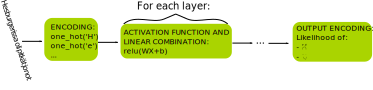
\includegraphics[width=0.9\textwidth]{./sentiment_analysis.png}

\end{frame}

\begin{frame}
\frametitle{Training Neural Networks}
\begin{itemize}
 \item In supervised training, the neural networks requires input and target output. The system finds a layered non-linear function from input to output.
 \item In unsupervised training, the network is only given input, and it learns a structure that captures the input statististical distributions and correlations.
 \item Unsupervised training uses energy-based methods which are better able to capture deep associations than a simple backpropagation, hence it is used for pre-training.
 \item A good platform to use for neural network experimentation is Google's TensorFlow, based on Python.
 \item Data representation is critical in neural networks, in the input representation, in the output representation (and by extension in defining the loss function), and
       also in the internal neuron representation.
\end{itemize}
\end{frame}

\begin{frame}
\frametitle{Tips \& Tricks}
 \begin{block}{Data Representation}
  \begin{itemize}
   \item Input representation
   \begin{itemize}
    \item Boolean values, Continuous values
    \item One-hot encoding for encoding exclusive choice
   \end{itemize}
   \item Output representation
   \begin{itemize}
    \item Boolean values, Continuous values
    \item One-hot encoding for encoding exclusive choice
    \item Mixture distributions
   \end{itemize}
   \item Internal representation
   \begin{itemize}
    \item Abstraction levels
    \item Bottlenecks and compression
   \end{itemize}
  \end{itemize}
 \end{block}
\end{frame}

\begin{frame}
\frametitle{Input Representation}
 \begin{itemize}
  \item One-hot 
 \end{itemize}
\end{frame}

\begin{frame}
\frametitle{Output Representation}
 \begin{itemize}
  \item 
 \end{itemize}
\end{frame}

\begin{frame}
\frametitle{Internal Representation}
 \begin{itemize}
  \item 
 \end{itemize}
\end{frame}

\begin{frame}
\frametitle{What did we learn?}
 \begin{itemize}
  \item To make neural networks learn effectively, the data must be represented in a suitable fashion.
 \end{itemize}
\end{frame}

\end{document}

